
\section{Elektronische Bauteile}

\subsection{Motor}\label{eb:motor}

% Tabelle
\begin{table}[!ht]
\centering
\rmfamily
\caption{Pinbelegung Motor}
\renewcommand{\arraystretch}{1.1}
\sffamily
\begin{footnotesize}
\begin{tabular}{r | l l}
\toprule
\textbf{Pin} & \textbf{Farbe}  & \textbf{Belegung}\\
\midrule
1 & Weiß & Motor +9V; PWM-Steuerung \\
2 & Schwarz & Motor -9V; PWM-Steuerung \\
3 & Rot & Ground \\
4 & Grün & +4,3V Versorgungsspannung \\
5 & Gelb & Motorencoder (Quadratur-Encoder, Kanal a) \\
6 & Blau & Motorencoder (Quadratur-Encoder, Kanal b) \\
\bottomrule
\end{tabular}
\end{footnotesize}
\label{eb:motor:tbl}
\end{table}

Die Steuerung des Motors erfogt über eine 9V Spannung. Für die Regulierung der Geschwindigkeit wird auf eine Pulsweitenmodulation zurückgeriffen. Die max. Stromstärke liegt bei 700mA für den Motor.  Die Versorgungsspannung an Pin 4 versorgt den Rotationssensor mit Strom. Mittels des Rotationssensors kann die genaue Rotationsposition des Motors bestimmt werden. Dieser Sensor kann über die Pin's 5 und 6 ausgelesen werden. Dieser Sensor wurde in diesem Projekt nicht weiter behandelt.


\subsection{Sensoren}\label{eb:sensor}


% Tabelle
\begin{table}[!ht]
\centering
\rmfamily
\caption{Pinbelegung Tastsensor}
\renewcommand{\arraystretch}{1.1}
\sffamily
\begin{footnotesize}
\begin{tabular}{r | l l}
\toprule
\textbf{Pin} & \textbf{Farbe}  & \textbf{Belegung}\\
\midrule
1 & Weiß & Trigger \\
2 & Schwarz & - \\
3 & Rot & Ground \\
4 & Grün & - \\
5 & Gelb & - \\
6 & Blau & - \\
\bottomrule
\end{tabular}
\end{footnotesize}
\label{tastsensor:tbl}
\end{table}
Der Tastsensor gehört zu den analog Sensorn vom NXT. Im Normalzustand ist der Tastsensor geöffnet (no: Normal Open). Die Leistungsaufnahme des Tastsensors ist im geöffneten zustand mit 2,2 mA sehr gering. Im geschlossenen Zustand liegt die Stromaufnahme bei 0 mA.



% Tabelle
\begin{table}[!ht]
\centering
\rmfamily
\caption{Pinbelegung Tonsensor}
\renewcommand{\arraystretch}{1.1}
\sffamily
\begin{footnotesize}
\begin{tabular}{r | l l}
\toprule
\textbf{Pin} & \textbf{Farbe}  & \textbf{Belegung}\\
\midrule
1 & Weiß & Analoges Tonsignal \\
2 & Schwarz & Ground \\
3 & Rot & Ground \\
4 & Grün & +4,3V Versorgungsspannung \\
5 & Gelb & Moduswahl dB/dBA \\
6 & Blau & Direkter Ausgang \\
\bottomrule
\end{tabular}
\end{footnotesize}
\label{tonsensor:tbl}
\end{table}
Der Tonsensor war nicht Teil dieses Projektes, jedoch wird er zur Vollständigkeit hier aufgeführt. Auch der Tonsensor ist ein Analogsensor. Dieser Senesor misst den Schalldruck zwischen 55 dB und 90 dB. Bei der Decibelskala ist zu beachten, dass es sich hier um eine Logarithmische Skalierung handelt. Somit nimmt der Mensch eine Erhöhung der Lautstärke um 10 dB als Verdopplung der Lautstärke wahr. Die Stromaufnahme des Tonsensors liegt bei 2,0 mA.
% Tabelle
\begin{table}[!ht]
\centering
\rmfamily
\caption{Pinbelegung Lichtsensor}
\renewcommand{\arraystretch}{1.1}
\sffamily
\begin{footnotesize}
\begin{tabular}{r | l l}
\toprule
\textbf{Pin} & \textbf{Farbe}  & \textbf{Belegung}\\
\midrule
1 & Weiß & Analoges Lichtsignal \\
2 & Schwarz & Ground \\
3 & Rot & Ground \\
4 & Grün & +4,3V Versorgungsspannung \\
5 & Gelb & Lichtquelle Ein/Aus \\
6 & Blau & - \\
\bottomrule
\end{tabular}
\end{footnotesize}
\label{lichtsensor:tbl}
\end{table}

Der Lichtsensor ist auch ein analoger Sensor. Über eine Lichtempfindlichen Widerstand (LDR) kann dieser Sensor die Helligkeit messen. Der Sensor hat zwei Modis. Der erste Modus ist \emph{Umgebungslicht Modus} mit einer Stromverbrauch von 2,5 mA.  Im \emph{Reflektions Modus} wird eine kleine LED aktiviert und der Stromverbrauch steigt so auf 15 mA.

% Tabelle
\begin{table}[!ht]
\centering
\rmfamily
\caption{Pinbelegung Ultraschallsensor}
\renewcommand{\arraystretch}{1.1}
\sffamily
\begin{footnotesize}
\begin{tabular}{r | l l}
\toprule
\textbf{Pin} & \textbf{Farbe}  & \textbf{Belegung}\\
\midrule
1 & Weiß & +9V Versorgungsspannung \\
2 & Schwarz & Ground \\
3 & Rot & Ground \\
4 & Grün & +4,3V Versorgungsspannung \\
5 & Gelb & I2C-Kommunikation SCL (Serial Clock) \\
6 & Blau & I2C-Kommunikation SDA (Serial Data) \\
\bottomrule
\end{tabular}
\end{footnotesize}
\label{eb:ultraschall:tbl}
\end{table}

Der ultraschall Sensor ist ein digitaler Sensor. Das bedeutet, dass das Signal mittels I2C-Bus übertragen wird. Mit diesem Sensor können Distanzen zwischen  0 cm und 255 cm gemessen werden. Es ist der einzigste Sensor der zusätzlich zu der normalen Versorgungsspannung von 4,3V noch eine 9V Versorgungsspannung benötigt.

\subsection{SN754410}\label{eb:pwm}
%Figure
\begin{wrapfigure}{r}{0.65\textwidth}
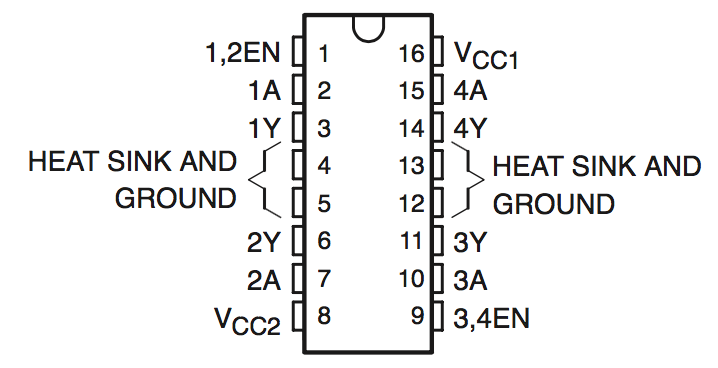
\includegraphics[width=0.9\linewidth]{bauelemente/sn754410}
\caption{SN754410}
\label{eb:fig:sn754410}
\end{wrapfigure}
Der SN754410 ermöglicht das Steuern der zwei Motoren mit einer max Stromstärke von 1 A (max Stromaufnahme eines Motors 700 mA) bei 9V. Die von uns  geschriebene Software steuert den Chip so an, dass über eine software Pulsweitenmodulation die Geschwindigkeit des Motors beliebig angepasst werden kann. Durch die Pulsweitenmodulation ist die Wärmeentwicklung sehr gering. Daher ist eine Kühlung dieses Bauteils nicht notwendig.

Über jeweils zwei GPIO-Pins kann so ein Motor gesteuert werden.

\subsection{MCP3008}\label{eb:adwandler}
%Figure
\begin{wrapfigure}{r}{0.4\textwidth}
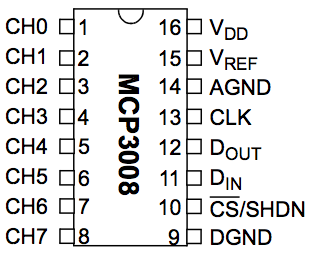
\includegraphics[width=0.9\linewidth]{bauelemente/mcp3008}
\caption{MCP3008}
\label{eb:mcp3008}
\end{wrapfigure}
Der MCP3008 ist ein Analog/Digital-Wandler (A/D-Wandler). Dieses Bauteil wird über den SPI-Bus am Raspberry Pi angeschlossen. Über den 8 Eingänge (CH0-CH7) lassen sich 8 verschiedene analoge Sensore anschließen. Der A/D-Wandler macht aus dem analogen Einganssignal einen Bitstream, der über den SPI-Bus übertragen wird.

Über vier GPIO-Pins können so 8 analoge Sensoren gesteuert werden.
